\documentclass[a4paper, 10pt]{report}

\usepackage{lipsum,lineno}
\usepackage{graphicx}
\usepackage{subcaption}
\usepackage{hyperref}
\usepackage{geometry}

\geometry{
	a4paper,
	total={170mm,257mm},
	left=22mm,
	top=22mm,
}

\title{App Report}
\author{Vibhor Porwal(160778)}
\date{}
\begin{document}
\maketitle

\listoffigures

\begin{figure}
\centering
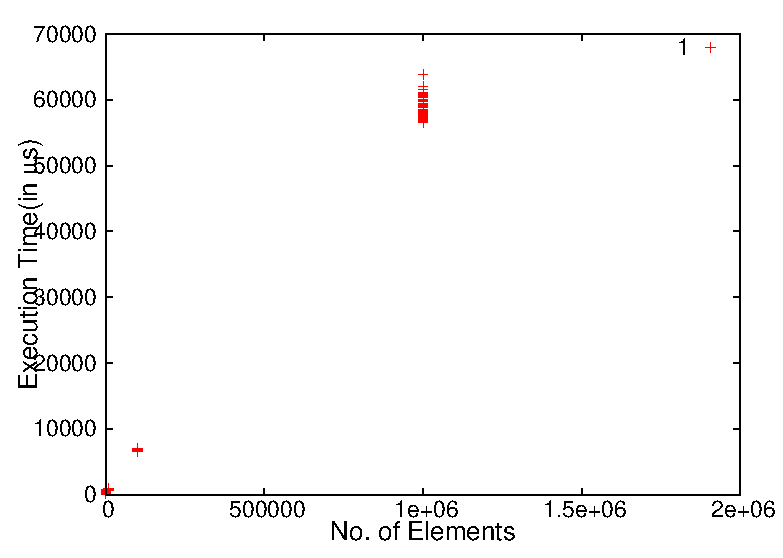
\includegraphics[width=\columnwidth]{thread1.eps}
\caption{Scatter Plot for No. of Threads 1}
\label{fig:thread1}
\end{figure}

\begin{figure}
\centering
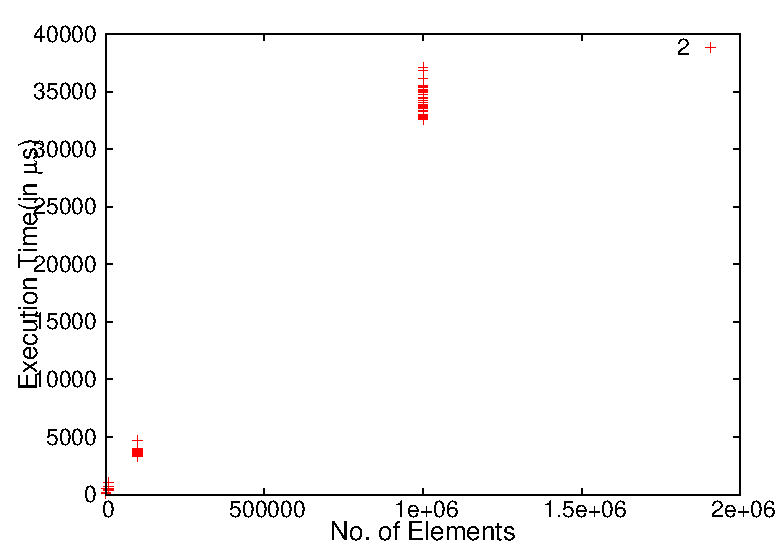
\includegraphics[width=\columnwidth]{thread2.eps}
\caption{Scatter Plot for No. of Threads 2}
\label{fig:thread2}
\end{figure}

\begin{figure}
\centering
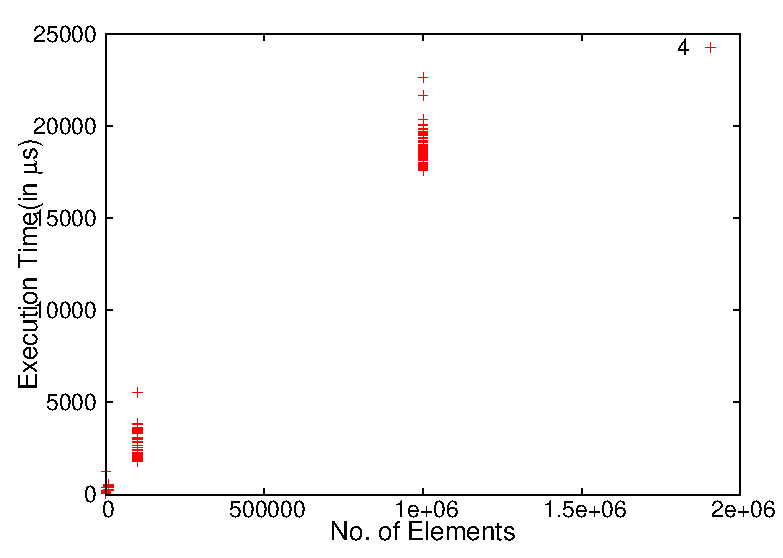
\includegraphics[width=\columnwidth]{thread4.eps}
\caption{Scatter Plot for No. of Threads 4}
\label{fig:thread4}
\end{figure}

\begin{figure}
\centering
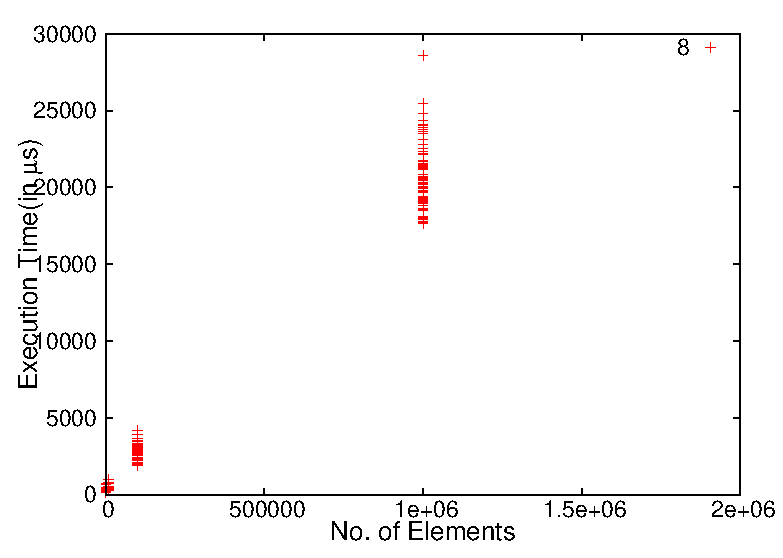
\includegraphics[width=\columnwidth]{thread8.eps}
\caption{Scatter Plot for No. of Threads 8}
\label{fig:thread8}
\end{figure}

\begin{figure}
\centering
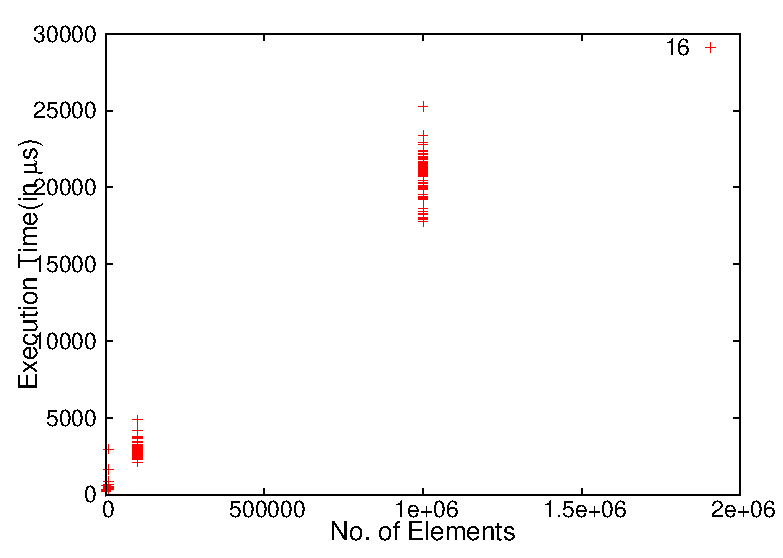
\includegraphics[width=\columnwidth]{thread16.eps}
\caption{Scatter Plot for No. of Threads 16}
\label{fig:thread16}
\end{figure}


\begin{figure}
\centering
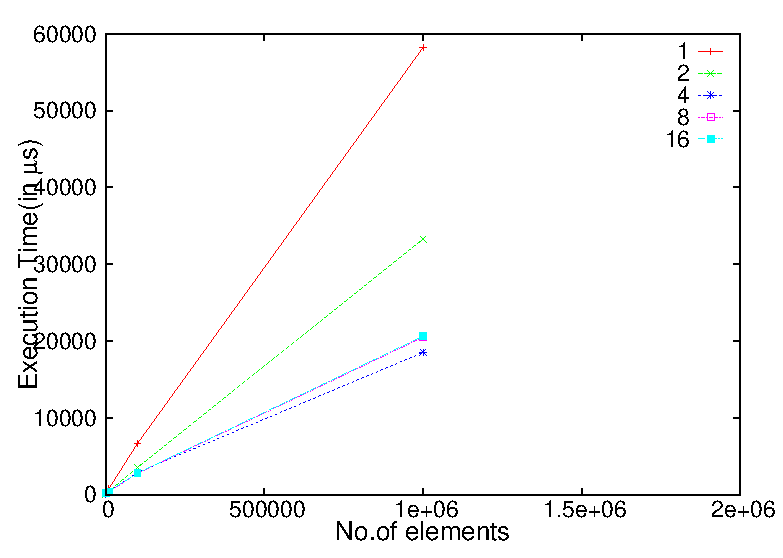
\includegraphics[width=\columnwidth]{line.eps}
\caption{Line Plot}
\label{fig:line}
\end{figure}

\begin{figure}
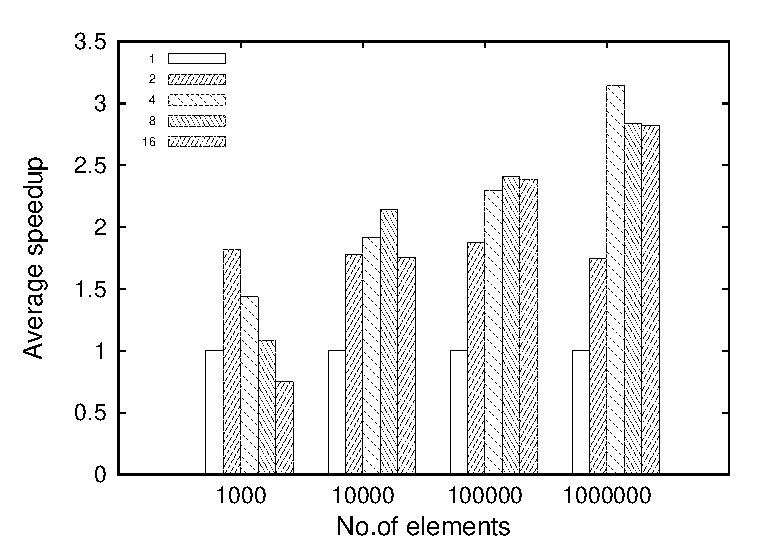
\includegraphics[width=\columnwidth]{bar.eps}
\caption{Avg Speedup Plot}
\label{fig:bar}
\end{figure}


\begin{figure}
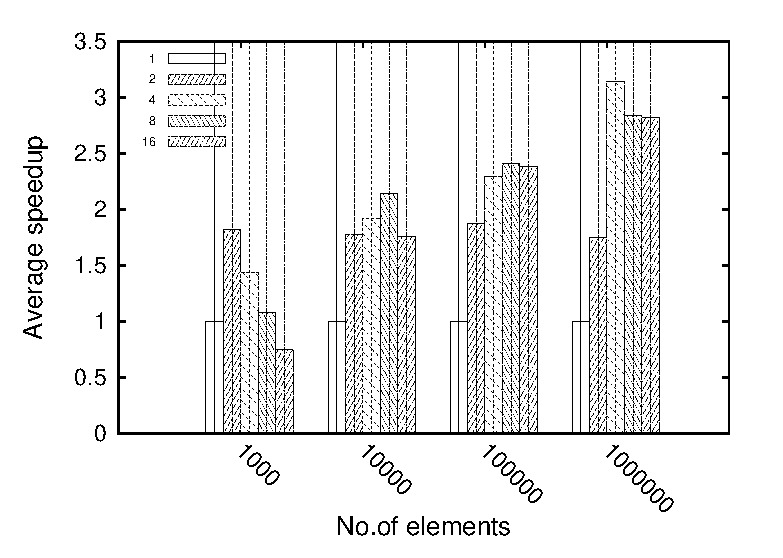
\includegraphics[width=\columnwidth]{error.eps}
\caption{ErrorBars}
\label{fig:errorbar}
\end{figure}


\end{document}
